\documentclass[twoside,a4paper,12pt]{article}
\usepackage{geometry}
\geometry{margin=1.5cm, vmargin={0pt,1cm}}
\setlength{\topmargin}{-1cm}
\setlength{\paperheight}{29.7cm}
\setlength{\textheight}{25.3cm}

% useful packages.
\usepackage{amsfonts}
\usepackage{amsmath}
\usepackage{amssymb}
\usepackage{amsthm}
\usepackage{enumerate}
\usepackage{graphicx}
\usepackage{multicol}
\usepackage{fancyhdr}
\usepackage{layout}
\usepackage{amsmath} 

% some common command
\newcommand{\dif}{\mathrm{d}}
\newcommand{\avg}[1]{\left\langle #1 \right\rangle}
\newcommand{\difFrac}[2]{\frac{\dif #1}{\dif #2}}
\newcommand{\pdfFrac}[2]{\frac{\partial #1}{\partial #2}}
\newcommand{\OFL}{\mathrm{OFL}}
\newcommand{\UFL}{\mathrm{UFL}}
\newcommand{\fl}{\mathrm{fl}}
\newcommand{\op}{\odot}
\newcommand{\Eabs}{E_{\mathrm{abs}}}
\newcommand{\Erel}{E_{\mathrm{rel}}}
\begin{document}

\pagestyle{fancy}
\fancyhead{}
\lhead{Jovi Wong(3180104829)}
\chead{Numerical Analysis homework \#3}
\rhead{2020/3/31}

\section*{I.A Min-Max Problem} 
We can define 
\begin{gather}
x=g(t)=(\frac{b-a}{2})t+(\frac{a+b}{2})\\
f(x)=a_0x^n+a_1x^{n-1}+\cdots+a_{n-1}x+a_n
\end{gather}
where $t \in [-1,1]$ and $x \in [a,b]$ , then
\begin{gather}
f(x)=f(g(t))=a_0g^n(t)+a_1g(t)^{n-1}+\cdots+a_{n-1}g(t)+a_n \\
=a_0[(\frac{b-a}{2})t+\frac{a+b}{2}]^n+a_1[(\frac{b-a}{2})t+\frac{a+b}{2}]^{n-1}+\cdots+a_{n-1}[(\frac{b-a}{2})t+\frac{a+b}{2}]+a_n\\
=b_0t^n+b_1t^{n-1}+\cdots+b_{n-1}t+b_n
\end{gather}
where $b_0=a_0[\frac{(b-a)}{2}]^n$, so
\begin{gather}
\min\max_{x\in[a,b]}|f(x)|=\min\max_{t\in [-1,1]}|b_0t^n+b_1t^{n-1}+\cdots+b_{n-1}t+b_n|\\
=|b_0|\min\max_{t\in [-1,1]}|t^n+\frac{b_1}{b_0}t^{n-1}+\cdots+\frac{b_{n-1}}{b_0}t+\frac{b_n}{b_0}|
\end{gather}
By Corollary 3.33,
\begin{gather}
\max_{t\in [-1,1]}|t^n+\frac{b_1}{b_0}t^{n-1}+\cdots+\frac{b_{n-1}}{b_0}t+\frac{b_n}{b_0}\geq \frac{1}{2^{n-1}}
\end{gather}
namely,
\[
|b_0|\min\max_{t\in [-1,1]}|t^n+\frac{b_1}{b_0}t^{n-1}+\cdots+\frac{b_{n-1}}{b_0}t+\frac{b_n}{b_0}|=\frac{|b_0|}{2^{n-1}}
\]
From above, we can draw the conclusion safely
\[
\min\max_{x\in[a,b]}|f(x)|=|a_0|\frac{(b-a)^n}{2^{2n-1}}
\]
\section*{II.Imitate the Proof of Cheybyshev Theorem}
Assume $\exists p(x) \in \overline{\mathbb{P}}^n$, such that 
\begin{gather}
\max_{x\in [-1,1]}p(x) < \max_{x\in[-1,1]}\frac{T_n(x)}{T_n(a)}
\end{gather}
Following Definition 3.28, it is obvious that
\begin{gather}
\max_{x\in[-1,1]}T_n(x)=1\\
\min_{x\in[-1,1]}T_n(x)=1
\end{gather}
Take (10) and (11) into (9), then we get
\begin{gather}
\max_{x\in [-1,1]}p(x) \leq \max_{x\in[-1,1]}|\frac{1}{T_n(a)}|
\end{gather}
We can define 
\begin{gather}
Q(x) = \frac{T_n(x)}{T_n(a)}-p(x)
\end{gather}
In particular, the property of $Q(x)$ worth noticing is that
\[
Q(a)=\frac{T_n(a)}{T_n(a)}-p(a)=0
\]
By Theorem 3.31,
\begin{gather}
Q(x'_k)=\frac{(-1)^k}{T_n(a)}-p(x'_k)
\end{gather}
The sigh of the sequence $\{Q(x'_i)\}_{i=1}^{n+1}$ is alternating, which means there are n zeros    of $Q(x)$ at least on $[a,b]$. Besides, there is another zero of $Q(x)$ on $x=a>1$. Therefore, the degree of $Q(x)$ is $n+1$ at least. Howerver, the degree of $T_n(x)$ and $p(x)$ is both $n$, which implies $Q(x)=0$, otherwise, it contrasts with the corollary we just get. The assumption is flase. Hence prove.
\section*{III.Programming}
\subsection*{b.Runge Phenomenon}
As the degree of interpolating polynomial increases, $\max{|f(x)-p(x)|}$ is also increses rapidly, especially near the beginning and ending points.
\begin{figure}[htbp]
 \centering
 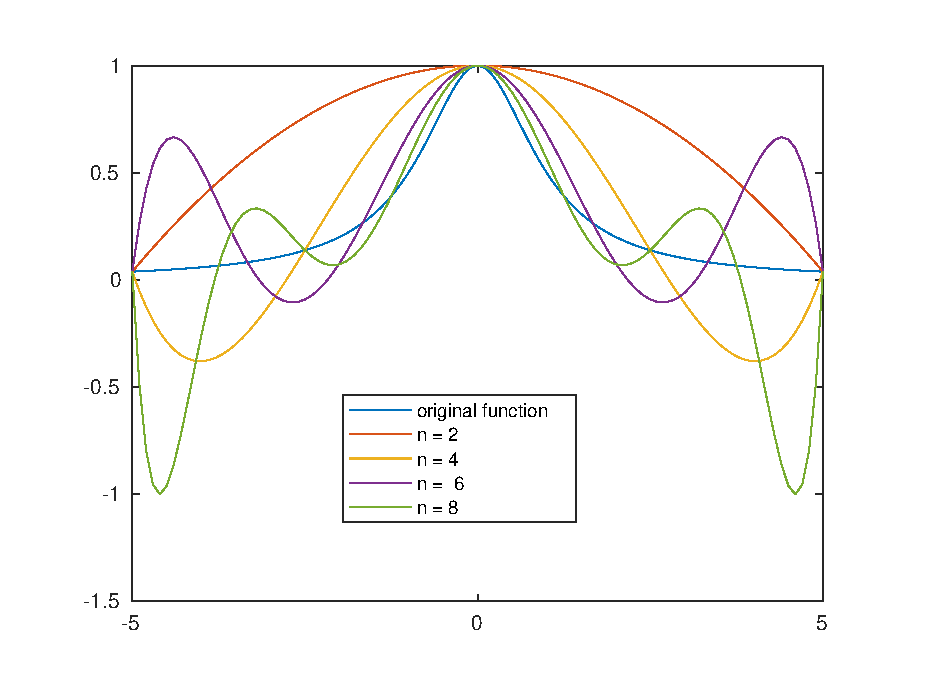
\includegraphics{NewtonPlot.eps}
 \caption{Newton Interpolation}
\end{figure}
\subsection*{c.Chebyshev Interpolation}

\begin{figure}
 \centering
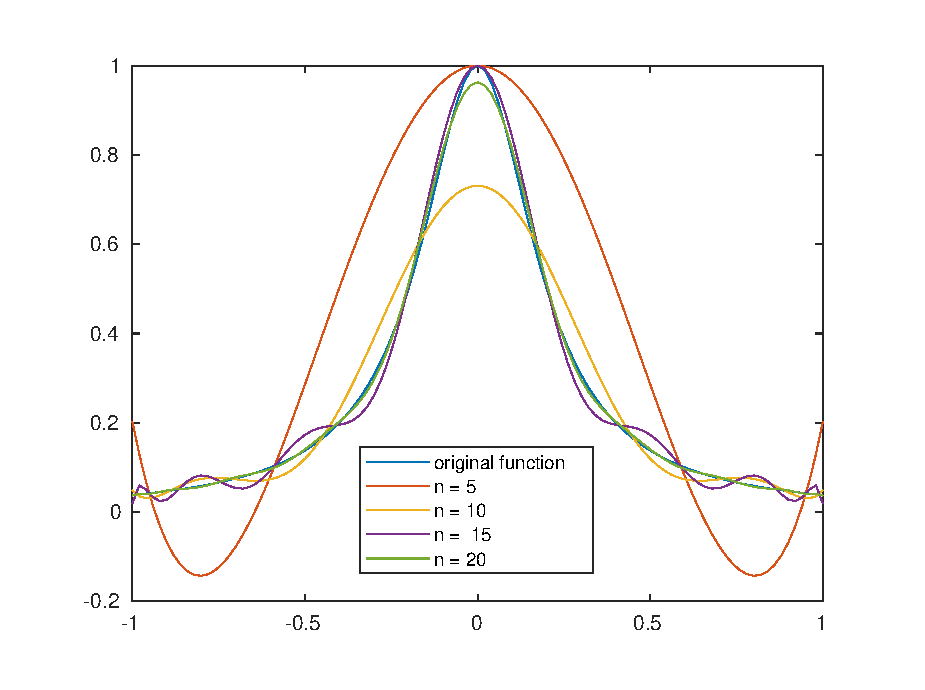
\includegraphics{ChebyshevPlot.eps}
 \caption{Chebyshev Interpolation}
\end{figure}
We can induce the following conclusion by Figure 2, 
\begin{gather}
\lim_{n\to \infty}\sup_{x\in[-1,1]}|f(x)-p_n(x)| = 0
\end{gather}
which implies the $\{p_n(x)\}$ converge to $f(x)$ uniformly.
\end{document}

%%% Local Variables: 
%%% mode: latex
%%% TeX-master: t
%%% End: 
